\documentclass[11pt]{article}
\pdfoutput=1 % tell arXiv's AutoTeX to compile with pdflatex

% --- arXiv-friendly preprint setup (plain article, no venue style) ---
\usepackage[margin=1in]{geometry}
\usepackage[utf8]{inputenc}
\usepackage[T1]{fontenc}
\usepackage{microtype}
\usepackage{graphicx}
\usepackage{booktabs}
\usepackage{float}
\usepackage{amsmath}
\usepackage{xcolor}
\usepackage[round]{natbib}
\usepackage[colorlinks=true, linkcolor=blue!60!black, citecolor=blue!60!black, urlcolor=blue!60!black]{hyperref}
\usepackage{caption}

\graphicspath{{figures/}}

% no single-line widows/orphans at page breaks
\widowpenalty=10000
\clubpenalty=10000
\displaywidowpenalty=10000

% TODO marker for drafting
\newcommand{\todo}[1]{\textcolor{red}{[TODO: #1]}}

\title{Measuring Drift in Therapeutic AI:\\
A Stability-Based Evaluation of Sovereign LLMs\\ in Nightmare Therapy}

\author{
  Daniel Menzel\\
  Institute of Cognitive Science, University of Osnabr\"uck\\
  \texttt{dmenzel@uos.de}
}

\date{July 2026}

\begin{document}
\maketitle

\begin{abstract}
More and more people turn to large language models for mental health support. The models respond fluently, but ask the same question twice and you may get two different answers. In therapy, where trust depends on predictable guidance, that variation changes the treatment a patient receives.

This paper measures response consistency in the rescripting phase of Imagery Rehearsal Therapy, where a model must choose a therapeutic strategy and carry it out. Twelve models, spanning the EU-sovereign Mistral family, two proprietary ceilings (GPT-5.4, Claude Sonnet~4.6), and open-weight comparators, are evaluated across 7{,}200 trials at five temperatures. Every trial sees a byte-identical frozen dialogue history, so any variation comes from the model alone. A three-level framework compares strategy selections (Jaccard similarity), response texts (BERTScore), and whether the model does what it declared (LLM-judge alignment, $\kappa = 0.777$ against human annotation).

The main findings are: (1)~Consistency differs by model far more than by patient. Median decision consistency spans 0.69 to 1.00 across models, while the six patient profiles show no significant effect. (2)~The instability sits in strategy selection, not execution. Temperature changes which strategies a model picks, not how well it carries them out. (3)~Greedy decoding is not reliably optimal. Ten of twelve models reach their best mean consistency at a low non-zero temperature, a pattern the small per-condition sample leaves suggestive rather than confirmed. (4)~BERTScore detects when the tone changes but not when the strategy does, so no single metric shows the full pattern. Mistral Medium~3.5, an EU-sovereign open-weight model, tops the overall stability ranking.
\end{abstract}

\section{Introduction}
\label{sec:intro}

Nightmare disorder affects roughly 4\% of adults \citep{sandman2013nightmares, li2010prevalence}, and Imagery Rehearsal Therapy (IRT) is its best-evidenced treatment \citep{krakow2001imagery, morgenthaler2018position}. Access, however, is scarce, motivating LLM-based delivery of structured protocols \citep{stade2024large, heinz2025randomized}. A therapeutic LLM must do more than produce plausible text: within a structured protocol it must make \emph{consistent clinical decisions} --- a patient re-entering the rescripting phase should not receive a confrontation strategy on one run and an avoidance-incompatible safety strategy on the next, purely by chance of sampling.

Existing evaluations of clinical LLMs focus on quality, safety, or efficacy of single outputs \citep{zhang2024psyeval, chiu2024computational}; run-to-run \emph{stability} at fixed input is rarely measured, despite growing evidence that sampling variance materially affects LLM behavior \citep{renze2024effect, novikova2025consistency}. \todo{Sharpen the gap statement against 2--3 closest works.}

\textbf{This paper.} We frame run-to-run consistency of clinical reasoning as a measurable property and evaluate it in the rescripting phase of IRT. Models declare their therapeutic strategy in a structured \texttt{<plan>} block before responding, enabling measurement at three levels: (1) \emph{plan consistency} --- pairwise Jaccard similarity of declared strategy sets; (2) \emph{response similarity} --- pairwise BERTScore of the therapeutic responses; (3) \emph{plan--response alignment} --- an LLM judge verifying that responses implement the declared strategies.

\textbf{Contributions.}
\begin{enumerate}
  \item A three-level, protocol-grounded stability evaluation framework for therapeutic LLMs, applied to the rescripting core of IRT with frozen dialogue histories as deterministic evaluation entry points.
  \item An empirical study of 11 models $\times$ 6 patient vignettes $\times$ 5 temperatures $\times$ 20 trials (6{,}600 trials), quantifying decision-level and response-level stability and their temperature dependence. \todo{one-sentence headline finding once results are final}
  \item An extensibility validation: Mistral Medium 3.5 was added post hoc, four months after the main runs, on identical frozen histories with a single configuration entry --- testing both the pipeline's extensibility claim and the robustness of the findings to model-set enlargement.
\end{enumerate}

\section{Related Work}
\label{sec:related}

\paragraph{IRT and digital delivery.} Imagery Rehearsal Therapy is the first-line psychological treatment for nightmare disorder \citep{krakow1995imagery, krakow2001imagery, morgenthaler2018position}, with rescripting as its cognitive core \citep{albanese2022nightmare}. Digital and conversational delivery of structured therapy protocols has shown feasibility \citep{fitzpatrick2017delivering, heinz2025randomized, wu2026pilot}. \todo{1--2 sentences tying reDreamAI / prior efficacy study (Llama 3.3 70B continuity).}

\paragraph{Evaluating clinical LLMs.} Existing frameworks target competence and safety of single responses \citep{zhang2024psyeval, chiu2024computational, iftikhar2025llm, stade2024large}; protocol fidelity instruments from clinical psychology \citep{mowbray2003fidelity, bellg2004enhancing, kohrt2015therapist} inspire our ternary alignment rubric. Our focus differs: not \emph{whether one response is good}, but \emph{whether repeated responses agree}.

\paragraph{LLM output consistency.} Sampling temperature and stochastic decoding measurably change task behavior \citep{renze2024effect}; recent work documents self-inconsistency across repeated runs \citep{novikova2025consistency, xu2025echoes, yuan2025understanding}. \todo{Position against these: none measure decision-level consistency in a clinical protocol.}

\paragraph{Chain-of-thought and declared intent.} CoT prompting \citep{wei2022chain} structures generation, but CoT explanations are often unfaithful to internal computation \citep{turpin2023language, lanham2023measuring}. We therefore frame the plan block as declared intent (Section~\ref{sec:plan}). LLM-as-judge protocols \citep{zheng2023judging} underpin Method~3, with cross-family judging to mitigate self-preference bias.

\section{Method}
\label{sec:method}

\subsection{Two-Stack Architecture}

The evaluation system separates dialogue creation from stability measurement (Figure~\ref{fig:pipeline}).
A \emph{generation stack} produces synthetic therapy sessions through a three-agent loop: a patient agent simulates responses based on a BDI-profiled vignette, a router agent classifies the current stage of the Imagery Rehearsal Therapy (IRT) protocol from the conversation history, and a therapist agent generates stage-appropriate responses. The loop traverses the five-stage IRT protocol (recording, rewriting, summary, rehearsal, final) and exports the dialogue as a \emph{frozen history}, together with prefixes sliced at rewriting-turn boundaries.

An \emph{evaluation stack} then measures stability on these frozen histories. The router is bypassed---the rescripting prompt is injected directly, since the protocol stage is known a priori---which isolates the therapist model from stage-classification error. Every trial receives byte-identical context: the frozen history sliced after the second rewriting exchange (slice~2), followed by the same rescripting instruction.

\begin{figure}[t]
  \centering
  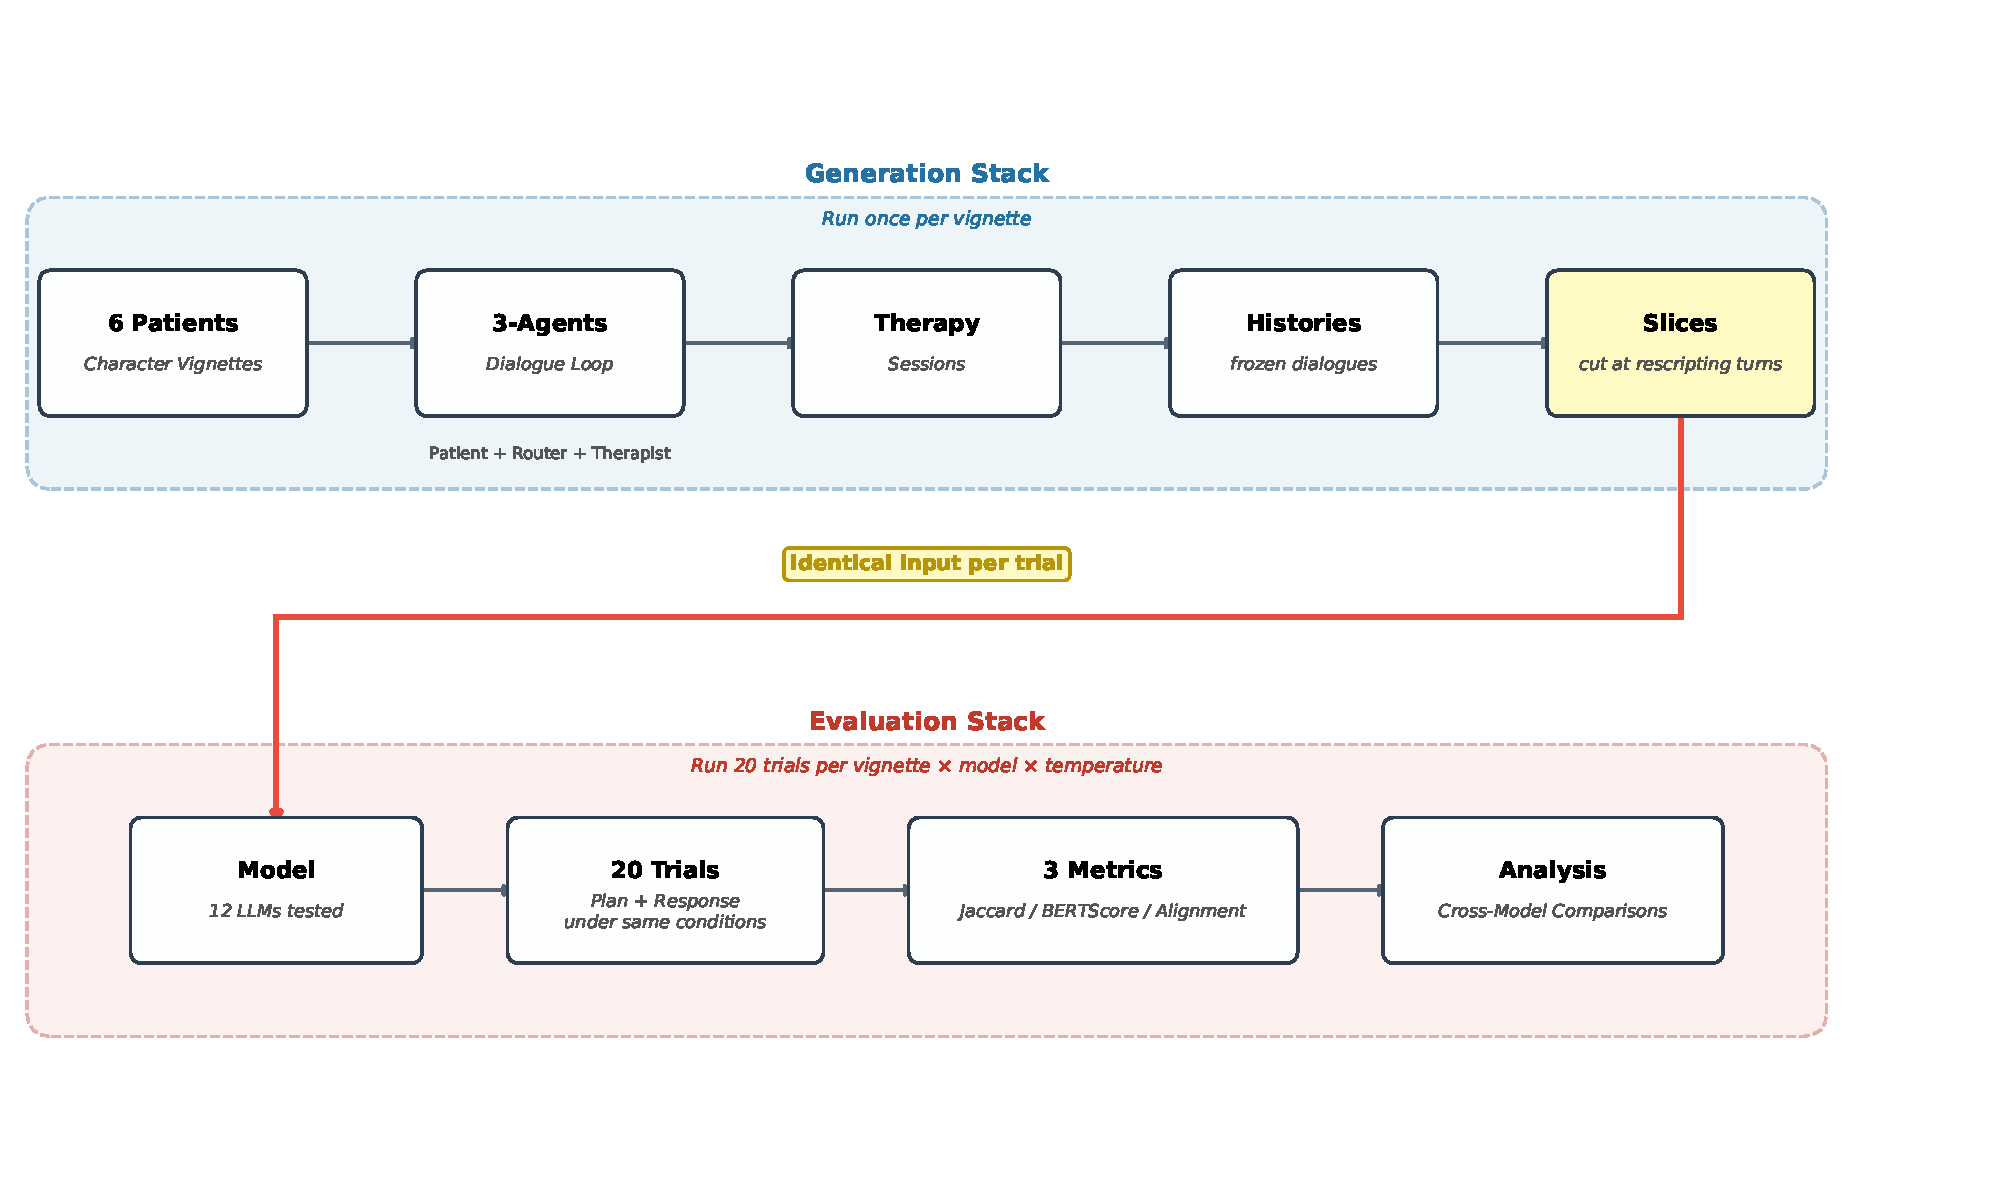
\includegraphics[width=\linewidth]{fig_3_1_pipeline}
  \caption{Pipeline overview: vignettes feed the generation stack; frozen histories feed the evaluation stack; each experiment run produces per-trial outputs and aggregated metrics.}
  \label{fig:pipeline}
\end{figure}

\subsection{The Plan Mechanism}
\label{sec:plan}

Each trial uses \emph{fused} chain-of-thought generation: the model first emits a plan block, \texttt{<plan>strategy\_1 / strategy\_2</plan>}, declaring one or two therapeutic strategies from a fixed taxonomy, then produces its therapeutic response in the same call, so the plan tokens condition the response tokens.

The plan block is a \emph{declared intent} mechanism, not a claim about internal reasoning. The chain-of-thought faithfulness debate \citep{turpin2023language, lanham2023measuring} is acknowledged but deliberately sidestepped: whether or not the declaration reflects internal computation, variable declarations predict variable clinical responses, and the declaration is what a clinical overseer would review.

\subsection{Strategy Taxonomy}
\label{sec:taxonomy}

Declarations are constrained to six categories describing concrete therapeutic \emph{mechanisms} (not goals): \texttt{confrontation} (external action toward the threat), \texttt{self\_empowerment} (internal transformation), \texttt{safety} (environment modification), \texttt{cognitive\_reframe} (meaning change), \texttt{social\_support} (adding allies), and \texttt{sensory\_modulation} (sensory and calming details). The taxonomy was refined over four iterations to resolve a severe distribution skew in which a single broad ``empowerment'' category absorbed 87.7\% of all picks; the final six categories are mechanism-level and mutually discriminable (Appendix~\ref{app:taxonomy}).

\subsection{Three Evaluation Metrics}
\label{sec:metrics}

Each experiment run consists of $N=20$ independent trials of one model on one vignette at one temperature. Three metrics target distinct layers of consistency (Figure~\ref{fig:measurement}):

\begin{figure}[t]
  \centering
  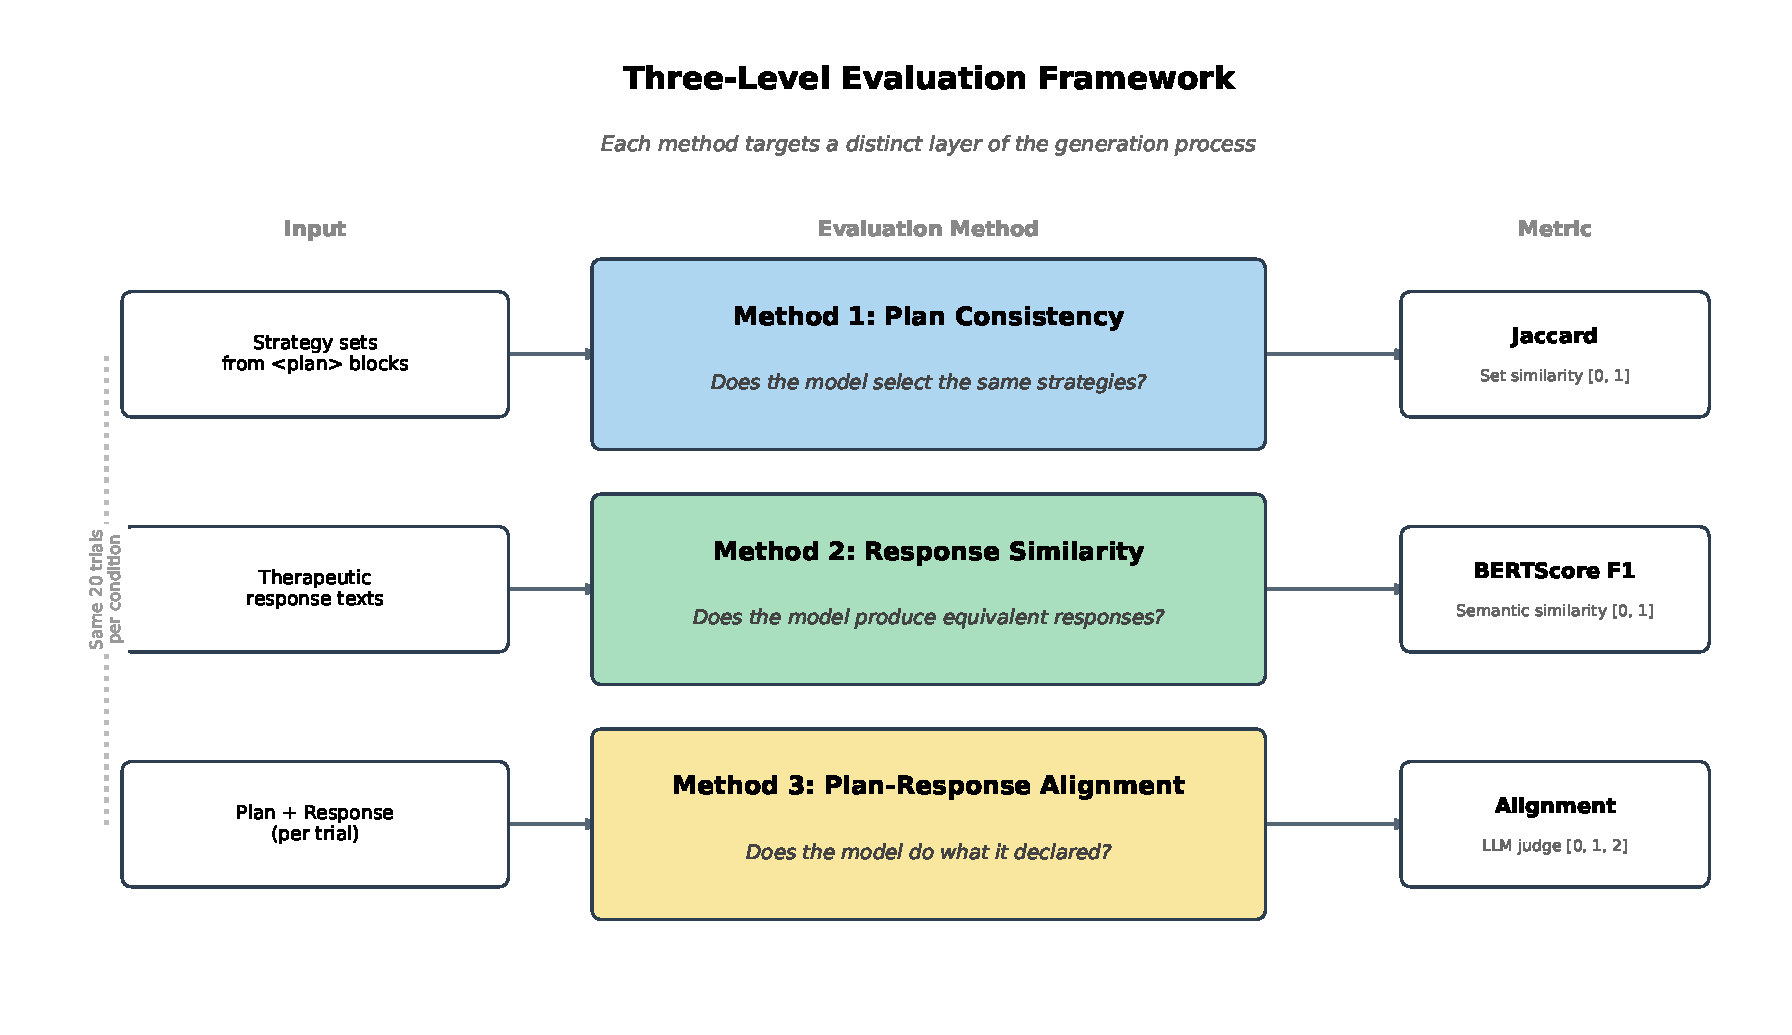
\includegraphics[width=\linewidth]{fig_3_2_measurement}
  \caption{The three-level measurement framework: each trial's output feeds plan consistency (Method~1), response similarity (Method~2), and plan--response alignment (Method~3).}
  \label{fig:measurement}
\end{figure}

\paragraph{Method 1: Plan consistency.} Do stochastic runs produce the same therapeutic \emph{decisions}? We compute the mean pairwise Jaccard similarity over the declared strategy sets across all $\binom{20}{2}=190$ trial pairs. A plan \emph{validity rate} (fraction of trials whose plan block parses to taxonomy categories) serves as an upstream quality gate.

\paragraph{Method 2: Response similarity.} Do stochastic runs produce therapeutically equivalent \emph{responses}? We compute mean pairwise BERTScore F1 \citep{zhang2020bertscore} over the response texts (plan blocks excluded) across the same 190 pairs, using DeBERTa-XLarge-MNLI \citep{he2021deberta} as the embedding model, which ranks first of 130+ models on WMT16 human correlation ($r=0.778$); its NLI fine-tuning aligns with the semantic-equivalence judgment the metric requires.

\paragraph{Method 3: Plan--response alignment.} Does the model \emph{do what it says}? An LLM judge (Gemini~3 Flash at $T{=}1.0$; suspect trials re-judged by Gemini~3.1 Pro) scores each declared strategy on a ternary scale (0 = absent, 1 = partial, 2 = implemented), normalized to $[0,1]$ per trial. Bias mitigations: cross-family judging (the judge's model family does not appear among evaluation targets), chain-of-thought justification, and a transparent rubric (Appendix~\ref{app:judge}). Judge trials that fail (timeout or API error) or are unjudgeable (invalid plan) are treated as missing data and excluded from the alignment mean rather than scored zero; invalid plans are already penalized by the validity rate.

Alignment primarily serves as a validation check: scores near the ceiling confirm that models implement what they declare, validating Jaccard as a measure of genuine decision stability rather than label noise.

\section{Experimental Setup}
\label{sec:setup}

\subsection{Models}
\label{sec:models}

EU data sovereignty is the primary selection criterion for the study's main subject: the reDreamAI deployment context requires a model that can be self-hosted within EU data residency boundaries \citep{dale2025sovereign}. The primary subject is therefore Mistral Large~3, the EU-sovereign Apache-2.0 flagship. Around it, the comparison set (Table~\ref{tab:models}) spans a size-class ladder from 24--32B dense models through 70B dense and 119--675B MoE up to two proprietary ceilings. Three scales of Qwen~3.5 probe within-family scaling, OLMo~3.1 provides full training-data provenance, and Llama~3.3~70B maintains continuity with the prior efficacy study. All models run in non-thinking mode via OpenRouter; Qwen~3.5 and Mistral Small~4 are hybrid-thinking models and run with reasoning disabled for fair comparison.

Mistral Medium~3.5 (128B dense, open weights under a modified MIT license, released 2026-04-30) was added \emph{post hoc} after the main data collection, using the identical frozen histories, prompts, and analysis pipeline. The addition serves two purposes: it tests whether the framework extends to a new model with a single configuration entry, and it tests whether the main findings are robust to enlarging the model set (Section~\ref{sec:robustness}).

\begin{table}[t]
  \centering
  \small
  \begin{tabular}{llll}
    \toprule
    Model & Size & Class & License \\
    \midrule
    Mistral Small 3.2 & 24B dense & small & Apache 2.0 \\
    Mistral Small 4 & 119B MoE (6.5B act.) & large MoE & Apache 2.0 \\
    Mistral Medium 3.5 & 128B dense & large dense & modified MIT \\
    Mistral Large 3 & 675B MoE (41B act.) & large MoE & Apache 2.0 \\
    Qwen 3.5 27B & 27B dense & small & Apache 2.0 \\
    Qwen 3.5 122B & 122B MoE (10B act.) & large MoE & Apache 2.0 \\
    Qwen 3.5 397B & 397B MoE (17B act.) & large MoE & Apache 2.0 \\
    OLMo 3.1 32B & 32B dense & small & Apache 2.0 (full provenance) \\
    Llama 3.3 70B & 70B dense & mid & Llama license \\
    GPT-5.4 & undisclosed & proprietary & --- \\
    Claude Sonnet 4.6 & undisclosed & proprietary & --- \\
    \bottomrule
  \end{tabular}
  \caption{Evaluation targets (therapist role). All models run in non-thinking mode via OpenRouter and were collected in March 2026, except Mistral Medium~3.5 (July 2026). Supporting roles are fixed across all runs: patient = Dolphin Mistral Venice 24B, router = Llama 3.3 70B, judge = Gemini 3 Flash with Gemini 3.1 Pro fallback (no family overlap with any evaluation target).}
  \label{tab:models}
\end{table}

\subsection{Conditions}

The full design crosses 11 models $\times$ 6 vignettes $\times$ 5 temperatures $\times$ 20 trials at slice~2, i.e.\ 600 trials per model and 6{,}600 trials in total.

The five-point temperature sweep, $T \in \{0.0, 0.075, 0.15, 0.3, 0.6\}$, is anchored in vendor documentation. $T{=}0.0$ (greedy decoding) serves as the deterministic reference, although GPU parallelisation leaves residual floating-point nondeterminism even there \citep{yuan2025understanding}, which the twenty-trial design captures directly \citep{blackwell2024towards}. $T{=}0.15$ is the Mistral vendor default. $T{=}0.6$ is the Qwen~3.5 and OLMo default, close to the standard Llama chat range and the proprietary defaults ($\approx 0.7$). $T{=}0.3$ fills the gap, and $T{=}0.075$ was added after an initial four-point run revealed that several models peak in consistency \emph{between} $T{=}0.0$ and $T{=}0.15$, a pattern examined in Section~\ref{sec:results-jaccard}.

No reproducibility seed was set, since not all vendors support one and even where available it is best effort at most. A supplementary experiment on Mistral Large~3 confirms this choice: fixing \texttt{seed=42} does not improve consistency over unseeded runs (Appendix~\ref{app:seed}). Trial repetition captures the stochastic variance directly.

\subsection{Statistical Analysis}
\label{sec:stats}

The analysis is primarily descriptive, and all tests are exploratory rather than confirmatory: the study describes stability patterns, it does not test a preregistered hypothesis. Spearman rank correlations quantify per-model temperature sensitivity and cross-metric relations (rank-based, because Jaccard takes few discrete values and BERTScore distributions may be non-normal). Kruskal--Wallis $H$ assesses model and vignette differences, with pairwise Mann--Whitney $U$ under Bonferroni correction ($\binom{11}{2}=55$ comparisons) and $\eta^2$ effect sizes alongside $p$-values.

No fixed threshold defines ``stable enough''; clinical significance thresholds for LLM stability do not yet exist. Results are interpreted comparatively, model against model and across the temperature sweep, with the random Jaccard baseline (expected value for random 2-of-6 selections, $\approx 0.2$) as the lower reference point.

\subsection{Reproducibility}

Model endpoints are pinned by OpenRouter model IDs; exact IDs, prompts, and aggregated per-condition results are released with the code at \url{https://github.com/me-daniel/measure-ai-drift}. The ten main models were collected between 2026-03-21 and 2026-03-24, Mistral Medium~3.5 on 2026-07-09, and a \texttt{run\_date} column in the released data records the collection date of every run. The frozen histories and per-trial raw outputs are retained by the author and available on request; a public release is planned. Two caveats: OpenRouter routes requests to third-party inference providers whose serving stacks (e.g.\ quantisation) may differ between requests and between the two collections, and the judge endpoints are versioned previews. Both are discussed in Section~\ref{sec:limitations}.

\section{Results}
\label{sec:results}

\todo{All numbers below from \texttt{stats/data/experiment\_test\_results.json} and \texttt{experiment\_descriptives.json} after the 11-model aggregation. Structure mirrors the thesis results chapter.}

\subsection{Plan Validity and Strategy Distribution}
\todo{validity rates per model (fig\_5\_1 / fig\_A1); strategy distribution across taxonomy.}

\subsection{Plan Consistency (Jaccard)}
\todo{fig\_5\_2 by family panels + fig\_5\_2b modal-set agreement; temperature trend; model differences w/ Kruskal--Wallis + Bonferroni pairwise.}

\subsection{Response Similarity (BERTScore)}
\todo{fig\_5\_3; compare decision-level vs response-level stability.}

\subsection{Vignette Effects}
\todo{fig\_5\_4.}

\subsection{Cross-Metric Relations}
\todo{fig\_5\_5; Spearman correlations between the three methods.}

\subsection{Plan--Response Alignment}
\todo{fig\_5\_6; alignment as validation check; report n\_judged fraction, pro-fallback fraction, and the missing-data rule for judge failures.}

\subsection{Robustness to Model-Set Enlargement: Mistral Medium 3.5}
\label{sec:robustness-results}

The post-hoc addition lands at the top of the stability ranking: Mistral Medium~3.5 attains a perfect median Jaccard of 1.000, the highest mean BERTScore F1 in the set (0.816), perfect plan validity (1.000), and mean alignment of 0.961 across its 30 conditions. Its Jaccard temperature profile stays at or near ceiling across all five temperatures.

Enlarging the pairwise family from $\binom{10}{2}=45$ to $\binom{11}{2}=55$ comparisons tightens the Bonferroni correction; exactly two marginal pairs among the original ten models lost significance (Jaccard: Llama~3.3~70B vs.\ Qwen~3.5~122B, $p_{\text{bonf}}$ $0.046 \to 0.056$; alignment: GPT-5.4 vs.\ Mistral Large~3, $0.045 \to 0.055$). No pairwise conclusion reversed direction, no pair became newly significant among the original ten, and the BERTScore pairwise structure is unchanged. All substantive findings of the original study hold under model-set enlargement.

\section{Discussion}
\label{sec:discussion}

\todo{Interpret: what do the stability levels mean for clinical deployment; temperature guidance; EU-sovereign subject vs proprietary ceiling verdict.}

\subsection{Robustness and Extensibility}
\label{sec:robustness}

Adding Mistral Medium~3.5 four months after the main data collection required a single configuration entry (model ID, temperature, reasoning mode) and one command; the 600-trial collection completed in roughly 8.5 hours of unattended wall-clock time on the identical frozen histories. No analysis code changed: aggregation, tests, and figures picked up the eleventh model automatically. The framework's extensibility is thus a demonstration rather than a claim, and the demonstration doubles as a robustness check --- Section~\ref{sec:robustness-results} shows all substantive findings survive the enlargement, with only two marginal Bonferroni boundary crossings. \todo{Optionally add API cost figure.}

\subsection{Limitations}
\label{sec:limitations}
\begin{itemize}
  \item \textbf{Synthetic patients.} Vignette-driven patient simulation, not clinical interactions.
  \item \textbf{Serving-stack variance.} OpenRouter routes to third-party providers; quantization and batching may differ between requests and between March and July collections.
  \item \textbf{Judge versioning.} Alignment scores depend on versioned Gemini preview endpoints; the judge for the July runs may differ in revision from March. Judge reliability is itself an open question \citep{zheng2023judging}.
  \item \textbf{Single protocol phase.} Rescripting only; stability elsewhere in IRT is unmeasured.
  \item \textbf{Exploratory statistics.} 30 runs per model; Bonferroni-corrected pairwise tests are conservative.
\end{itemize}

\section{Conclusion}
\label{sec:conclusion}

This paper asked how consistent LLM therapeutic responses are across independent runs within a structured IRT protocol. Three evaluation methods were applied to twelve models across 7{,}200 trials spanning five temperature conditions, on frozen histories that make every trial's input byte-identical.

The main findings are:

\begin{enumerate}
  \item Consistency varies widely across models and far less across patients. Median decision consistency spans 0.69 to 1.00 between models, while the vignette effect is not significant. Stability is a model property.
  \item The instability sits in strategy selection, not execution. Temperature reduces plan consistency but not plan--response alignment: models pick different strategies at higher temperatures but carry out whichever strategy they pick equally well.
  \item Greedy decoding is not always optimal. Ten of twelve models reach their best mean consistency at a low non-zero temperature, and the Mistral family peaks at its vendor default. Deployments should verify stability at the vendor-recommended setting rather than assume $T{=}0.0$ is safest.
  \item No single metric captures the full picture. The three levels correlate only moderately ($\rho = 0.29$ to $0.55$). BERTScore misses strategy changes and overstates drift from harmless paraphrase, and only the combination localises where instability lives.
  \item The framework is cheap to extend, and the findings are robust to model-set changes. Adding a model requires a single configuration entry on identical frozen inputs, the framework's own stability signature exposed a gateway silently dropping GPT-5.4's temperature parameter, and every substantive finding holds across these revisions. Mistral Medium~3.5, an EU-sovereign open-weight model, tops the overall stability ranking.
\end{enumerate}

The three-level framework fulfilled its design goal by identifying that instability concentrates at the strategy selection layer. Neither BERTScore nor alignment alone would have revealed that. The cross-model comparison shows that EU-sovereign deployment no longer requires a stability compromise: what was a small gap for Mistral Large~3 at its recommended temperature became, with Mistral Medium~3.5, the top of the ranking.

Several directions follow. Extending the evaluation beyond the rescripting phase would test whether the patterns hold across different types of clinical decisions, and the framework transfers to other manualised protocols (CBT, motivational interviewing) given a protocol-specific taxonomy. Since vendors update weights and serving infrastructure without notice, repeating the evaluation across model versions would show whether stability improves or fluctuates over release cycles. reDreamAI targets German-speaking users, so evaluating stability in German would test whether the English-language patterns transfer. A larger human annotation study would strengthen the judge validation beyond the current 60-trial subset. Finally, because consistency is necessary but not sufficient, the natural companion to this framework is an evaluation of therapeutic quality: a model must make the same decision every time, and it must be the right one.


\section*{Ethics Statement}
All patient interactions in this study are simulated. The six patient vignettes are synthetic behavioural profiles, no human participants were involved, and no real patient data were processed. The vignette design was informed by anonymised session data from a prior efficacy study, but no real transcripts were used. The results measure computational consistency, not clinical safety or efficacy, and do not support deploying any evaluated model to real patients without clinical validation.

\bibliographystyle{plainnat}
\bibliography{references}

\appendix
\section{Strategy Taxonomy}
\label{app:taxonomy}
\todo{Taxonomy card: six categories with definitions and example phrases; brief evolution note (8 $\to$ 6 $\to$ 7 $\to$ 6, skew collapse figure).}

\section{Prompts}
\label{app:prompts}
\todo{Rescripting prompt, fused-generation instruction, vignette example.}

\section{Judge Rubric}
\label{app:judge}
\todo{Judge system prompt, ternary rubric, example judgment with CoT justification; missing-data rule for judge failures.}

\section{Per-Condition Results}
\label{app:tables}
\todo{Full 11-model $\times$ 5-temperature tables for all three metrics.}


\end{document}
